\chapter{Usability}\label{ch:usability}

In diesem Kapitel wird die Usability anhand eines Usability Tests getestet.
Bei den Tests wird sich zur Vereinfachung der Vergleichbarkeit aud die Seiten google.de, bing.de, qwant.de beschränkt.
Auch wird sich bei der Einhaltung von Regeln und Gesetzen auf das deutsche Recht beschränkt.

\section{Test-Szenarien}\label{sec:szenarien}
Zur Durchführung wurden eine kleine Gruppe Informatik Studenten der \textbf{DHBW} gewählt.
Aufgrund mangelnder Ressourcen wurden diese in Eigenregie und ohne erstrebenswerte Tracking-Technologien wie z.B.\ Eye-tracking oder ähnliches durchgeführt.
Die Tester haben die Szenarien mit den drei verschiedenen Suchmaschinen \url{google.de} \url{bing.de} \url{qwant.de} durchgeführt,
und die Ergebnisse nach vorgegebenem Schema auf einer Skala von 1 bis 10 bewertet.

\subsection{Tag des Internets}\label{subsec:szenario1}
In diesem Szenario bekamen die Tester den Auftrag herauszufinden, wann der Tag des Internets ist.

\begin{tabular}{|c|c|c|c|}
    \hline
    & Dauer & Ergebnis & Selbsteinschätzung \\
    \hline
    Google & 10    & 10       & 10                 \\
    \hline
    Bing   & 9     & 9        & 8                  \\
    \hline
    Qwant  & 9     & 4        & 7                  \\
    \hline
\end{tabular}

\subsubsection*{Auswertung}
\paragraph{\url{google.de}}
hat durch die in der Mitte liegende Suchbar und das minimalistische Design,
sowie der sowieso sehr hohen Popularität eine schnelle Bedienbarkeit besonders bei einfachen Suchanfragen.\\

\paragraph{\url{bing.de}} hat durch die nicht ganz zentrale Suchleiste und das Design mit farbigem Hintergrundbild etwas länger gebraucht bis die Tester sich orientieren konnten.
Die Ergebnisseite von \url{google.de} und \url{bing.de} sind sich sehr ähnlich, siehe\nameref{fig:tag_des_internets_results}, weshalb dort auch von den Testern keine nennenswerten Unterschiede festzustellen waren.\\
\begin{figure}
    \centering
    \begin{minipage}[t]{0.45\linewidth}
        \centering
        \fbox{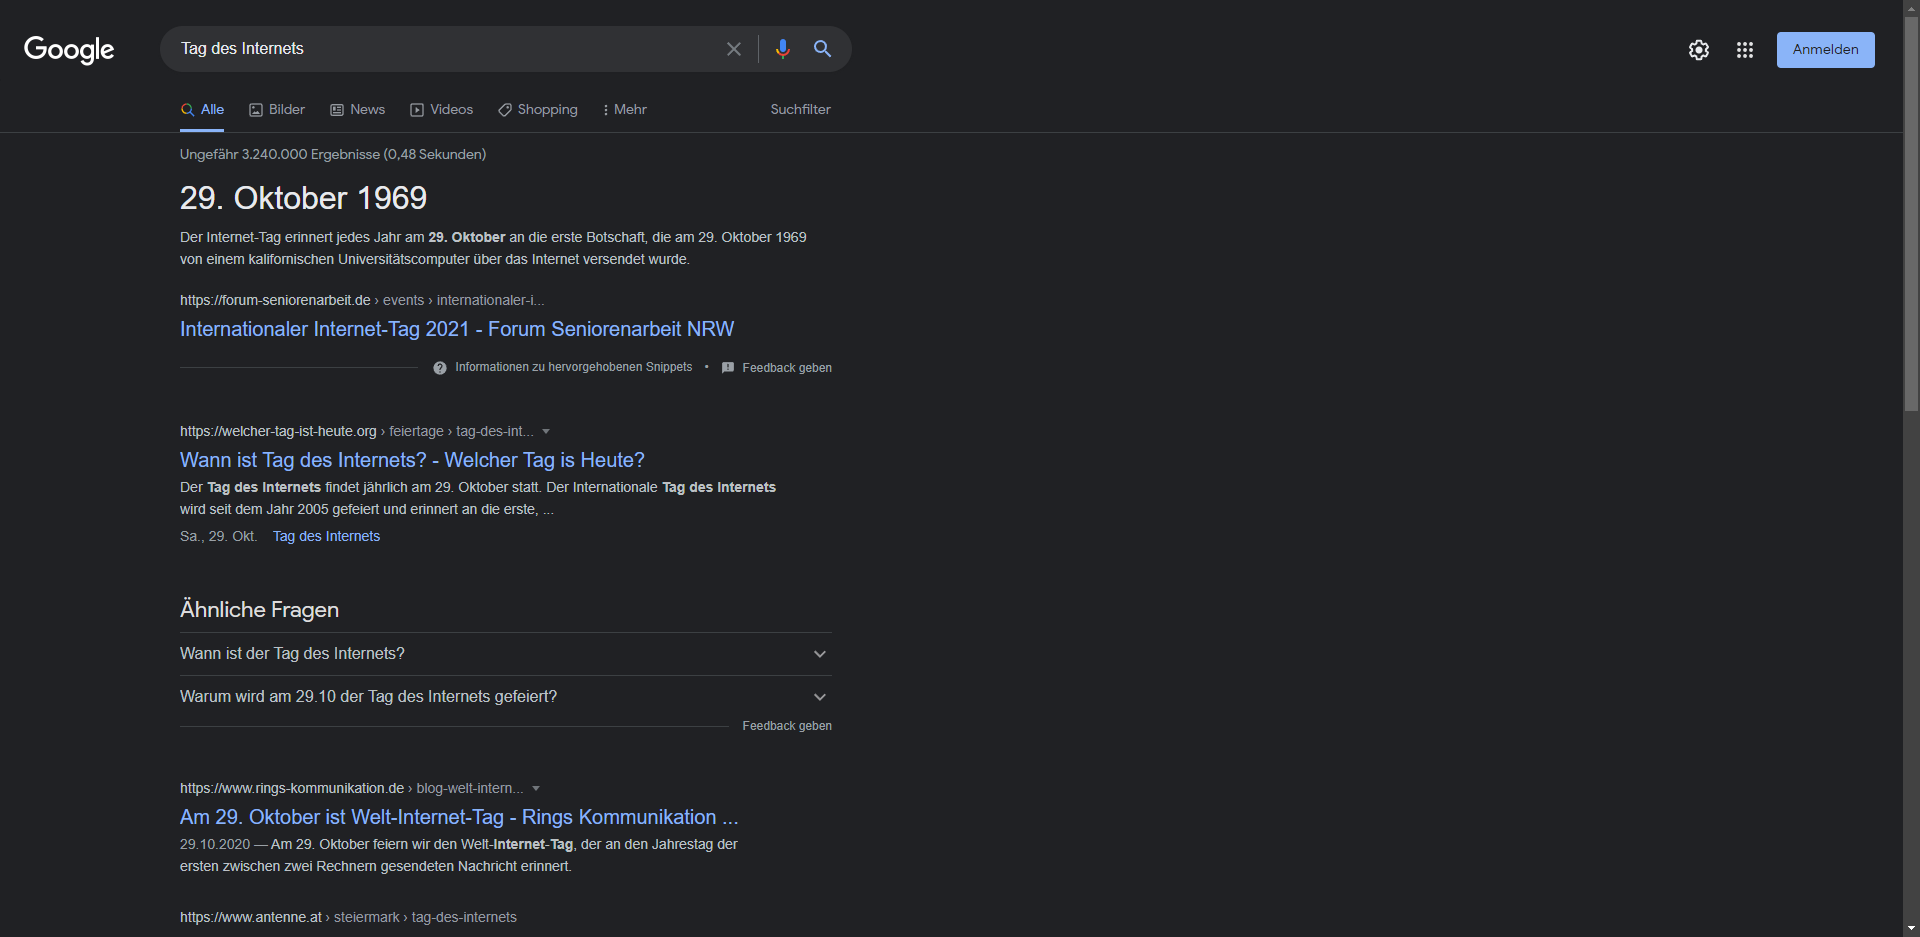
\includegraphics[width=\linewidth]{google_tag_des_internets_results}}
        Ergebnisse von \url{google.de}
    \end{minipage}%
    \hfill\vrule\hfill
    \begin{minipage}[t]{0.45\linewidth}
        \centering
        \fbox{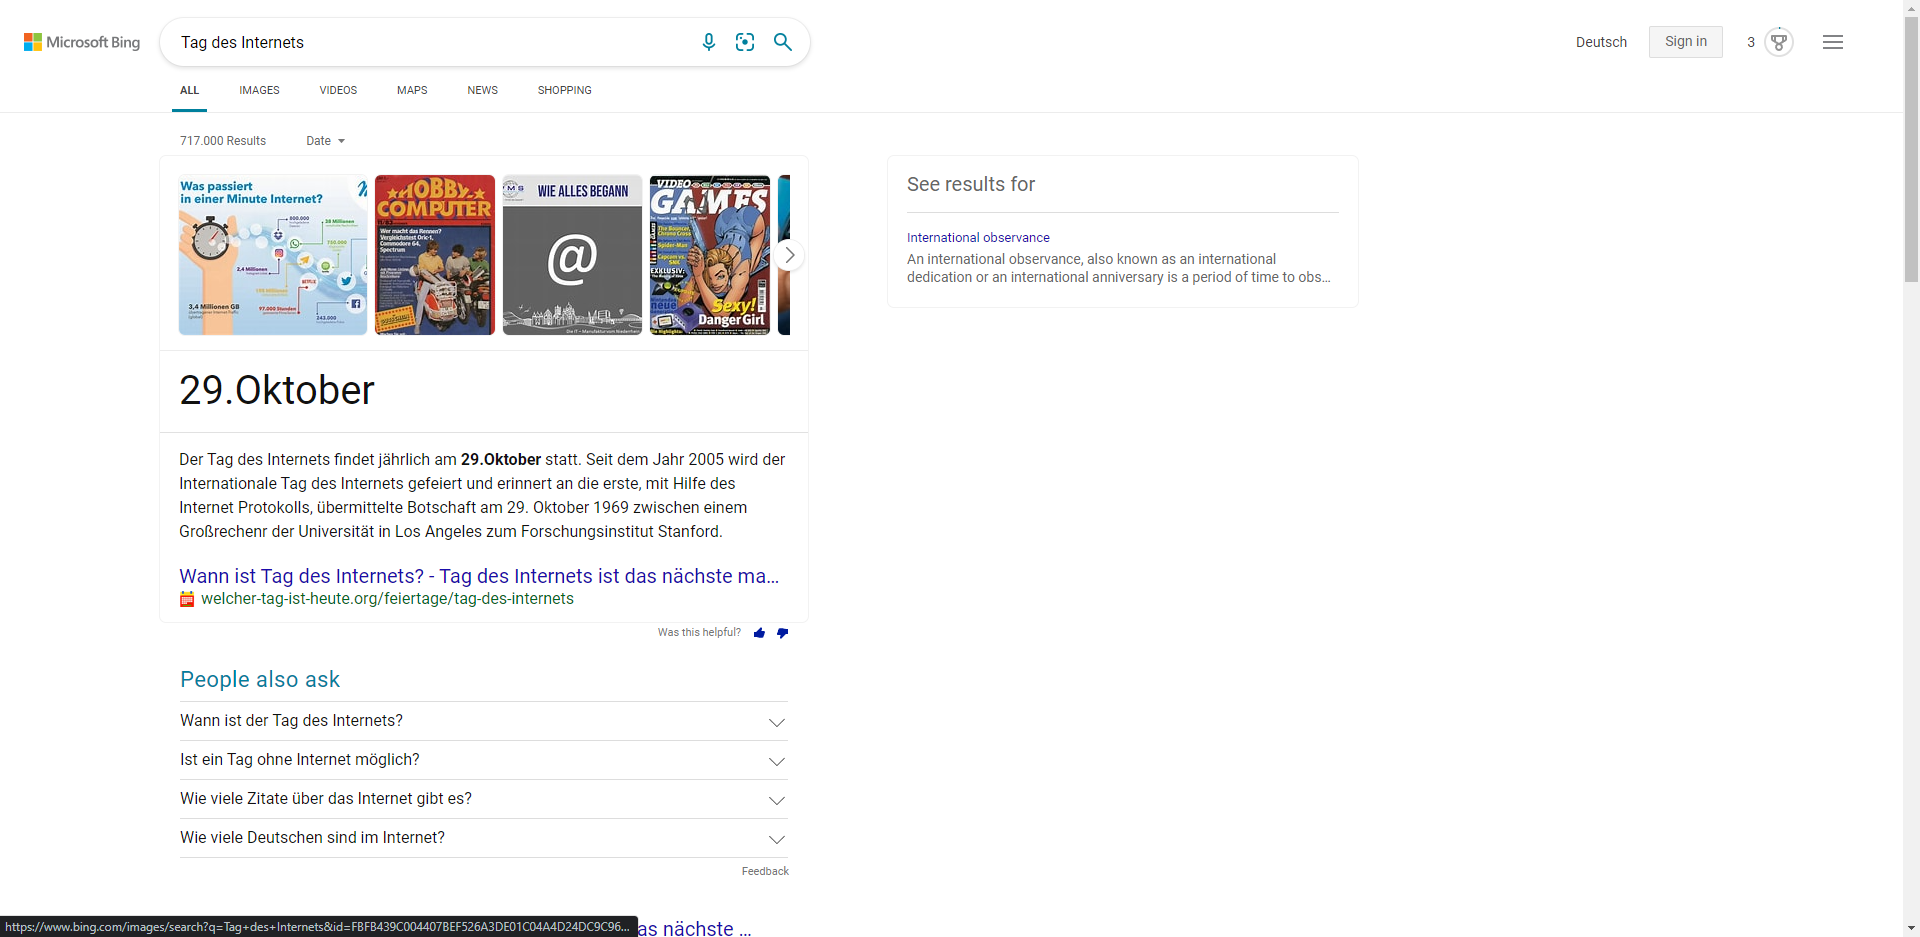
\includegraphics[width=\linewidth]{bing_tag_des_internets_results}}
        Ergebnisse von \url{bing.de}
    \end{minipage}
    \caption{Vergleich Ergebnis Google und Bing}\label{fig:tag_des_internets_results}
\end{figure}

\paragraph{\url{qwant.de}} hat bei den Testern eine lange Zeit gebraucht, um sich zu orientieren,
da das Design mit grellen Farben den Blick in die Mitte des Bildschirms gelockt hat und auch mehrere Knöpfe und Auswahlmöglichkeiten existieren.
Die hat es laut Aussagen der Tester erschwert, die Suchleiste in etwas dunklerem Design am oberen Bildschirmrand zu finden.
Auch die~\nameref{fig:qwant_tag_des_internets_results} ist nicht so gut wie bei \url{google.de} oder \url{bing.de},
da eine Übersicht mit dem Datum nicht direkt auf der Seite zu finden ist,
sondern erst in den Ergebnisseiten zu finden ist
\begin{figure}
    \centering
    \fbox{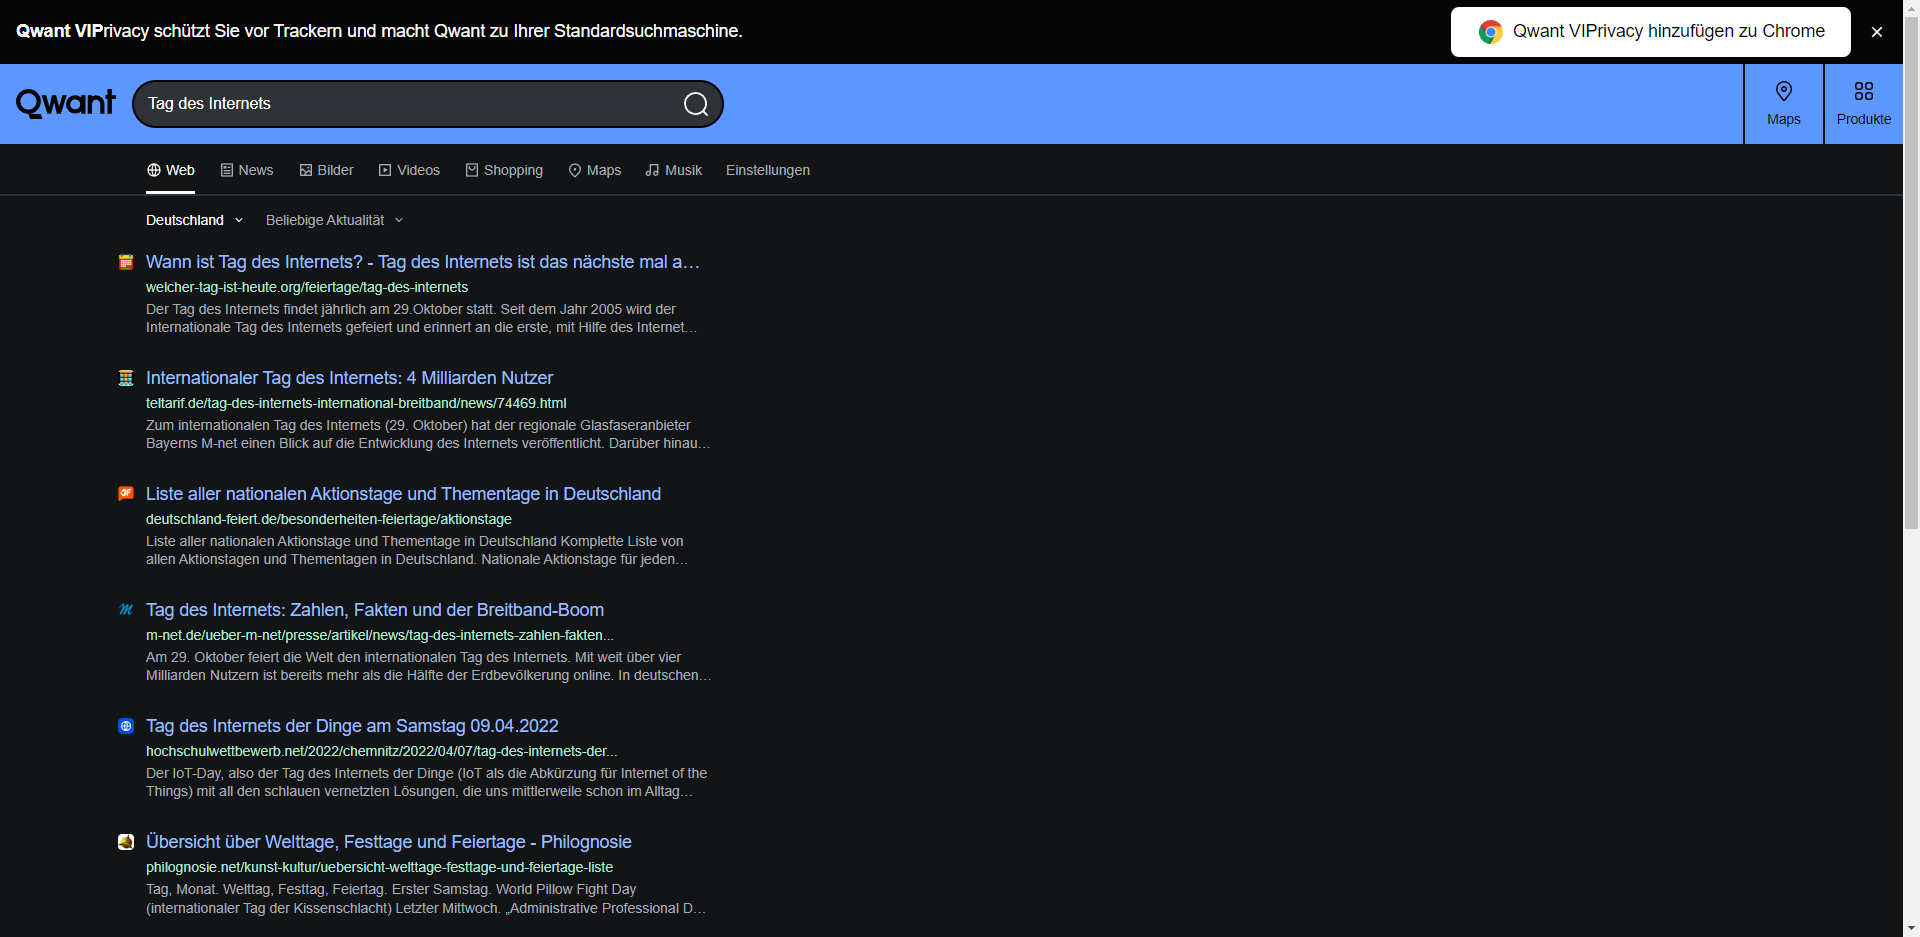
\includegraphics[width=0.5\linewidth]{qwant_tag_des_internets_results}}
    \caption{Ergebnisseite von \url{qwant.de}}\label{fig:qwant_tag_des_internets_results}
\end{figure}

\subsection{Katzenbild}\label{subsec:szenario2}
In diesem Szenario bekamen die Tester den Auftrag ein Katzenbild zu finden.

\begin{tabular}{|c|c|c|c|}
    \hline
    & Dauer & Ergebnis & Selbsteinschätzung \\
    \hline
    Google & 9     & 8        & 9                  \\
    \hline
    Bing   & 9     & 9        & 9                  \\
    \hline
    Qwant  & 10    & 10       & 10                 \\
    \hline
\end{tabular}

\subsubsection*{Auswertung}
%TODO Auswertung

\subsection{Songtext}\label{subsec:szenario3}
In diesem Szenario bekamen die Tester den Auftrag den Songtext des Lieds Never gonna give you up von Rick Astley zu finden.

\begin{tabular}{|c|c|c|c|}
    \hline
    & Dauer & Ergebnis & Selbsteinschätzung \\
    \hline
    Google & 8     & 10       & 7                  \\
    \hline
    Bing   & 6     & 5        & 6                  \\
    \hline
    Qwant  & 6     & 5        & 6                  \\
    \hline
\end{tabular}

\subsubsection*{Auswertung}
%TODO Auswertung

\section{Accessibility}\label{sec:accessibility}
In diesem Kapitel wird die Accessibility getestet.
Es gibt einige Tests, die manuell und aufwändig getestet werden müssen.
Diese wurden nicht durchgeführt und es wurde sich auf die Ergebnisse der automatisierten Tests beschränkt.

Es werden die Guidelines der Web Accessibility Initiative (WAI) verwendet.
Diese Guidelines sind auf der Seite \url{https://www.w3.org/WAI/standards-guidelines/wcag/} verfügbar.\newline
Es wird unterschieden in folgende Level~\cite{WCAG21}:
\begin{itemize}
    \item Level A: niedrigstes Level der Accessibility.
    \item Level AA: mittleres Level der Accessibility.
    \item Level AAA: höchstes Level der Accessibility.
\end{itemize}

%TODO link to appendix

\subsection{Google}\label{subsec:google}
Wie in der Auswertung des Accessibility-Tests zu sehen ist, hat \url{google.de} mehrere Probleme mit der Accessibility.
Davon sind folgende Probleme als kritisch bewertet:
\begin{enumerate}
    \item Ein Button hat keinen besonderen Namen bekommen, wodurch es für Screenreader nicht möglich ist den Nutzern die Funktion des Buttons mitzuteilen.
    \item Der Kontrast zwischen Hintergrund und Vordergrund ist nicht ausreichend.
\end{enumerate}
Diese Probleme sind zwar als kritisch markiert, das Problem mit dem Button ist aber bei mehrfachen Tests nicht mehr aufgetreten.
Da minimale Kontraste in den WCAG 2.1-Guidelines erst für Level AA vorgeschrieben sind ist dies nicht fatal, sollte jedoch für ein Unternehmen wie Google durchaus erstrebenswert sein,
um die Benutzbarkeit für Menschen mit Sehbehinderung zu verbessern.

\subsection{Bing}\label{subsec:bing}
Wie in der Auswertung des Accessibility-Tests zu sehen ist, hat \url{bing.de} ein Problem mit der Accessibility.
Folgendes Problem wurde als kritisch bewertet:
\begin{enumerate}
    \item Die Zoomfunktion wurde in den meta-Tags deaktiviert.
\end{enumerate}
Dieses Problem scheint jedoch nur das Hintergrundbild zu betreffen, da das Interface vergrößert werden kann.
Aus diesem Grund ist das Problem als nicht kritisch zu betrachten, da die Benutzbarkeit für Menschen mit Sehbehinderung nicht beeinträchtigt wird.

\subsection{Qwant}\label{subsec:qwant}
Wie in der Auswertung des Accessibility-Tests zu sehen ist, hat \url{qwant.de} Probleme mit der Accessibility.
Folgende Probleme wurden als kritisch bewertet:
\begin{enumerate}
    \item Ein Button hat keinen besonderen Namen bekommen, wodurch es für Screenreader nicht möglich ist den Nutzern die Funktion des Buttons mitzuteilen.
    \item Der Linktext einiger Elemente ist nicht eindeutig.
\end{enumerate}
Das Problem mit den Nicht eindeutig benannten Elementen ist auch bei mehrfachen Tests aufgetreten.
Da eindeutige Namen in den WCAG 2.1-Guidelines für Level A vorgeschrieben sind siehe `Success Criterion 1.1.1 Non-text Content`\cite{WCAG21},
ist dies eine klare Verletzung der WCAG 2.1 A Guidelines, wodurch sich \url{qwant.de} nicht für eine Accessibility-Kompatibilität laut WCAG 2.1-Guidelines qualifiziert.

\section{Vergleich}\label{sec:vergleich}
\begin{figure}[h]
    \centering
    \fbox{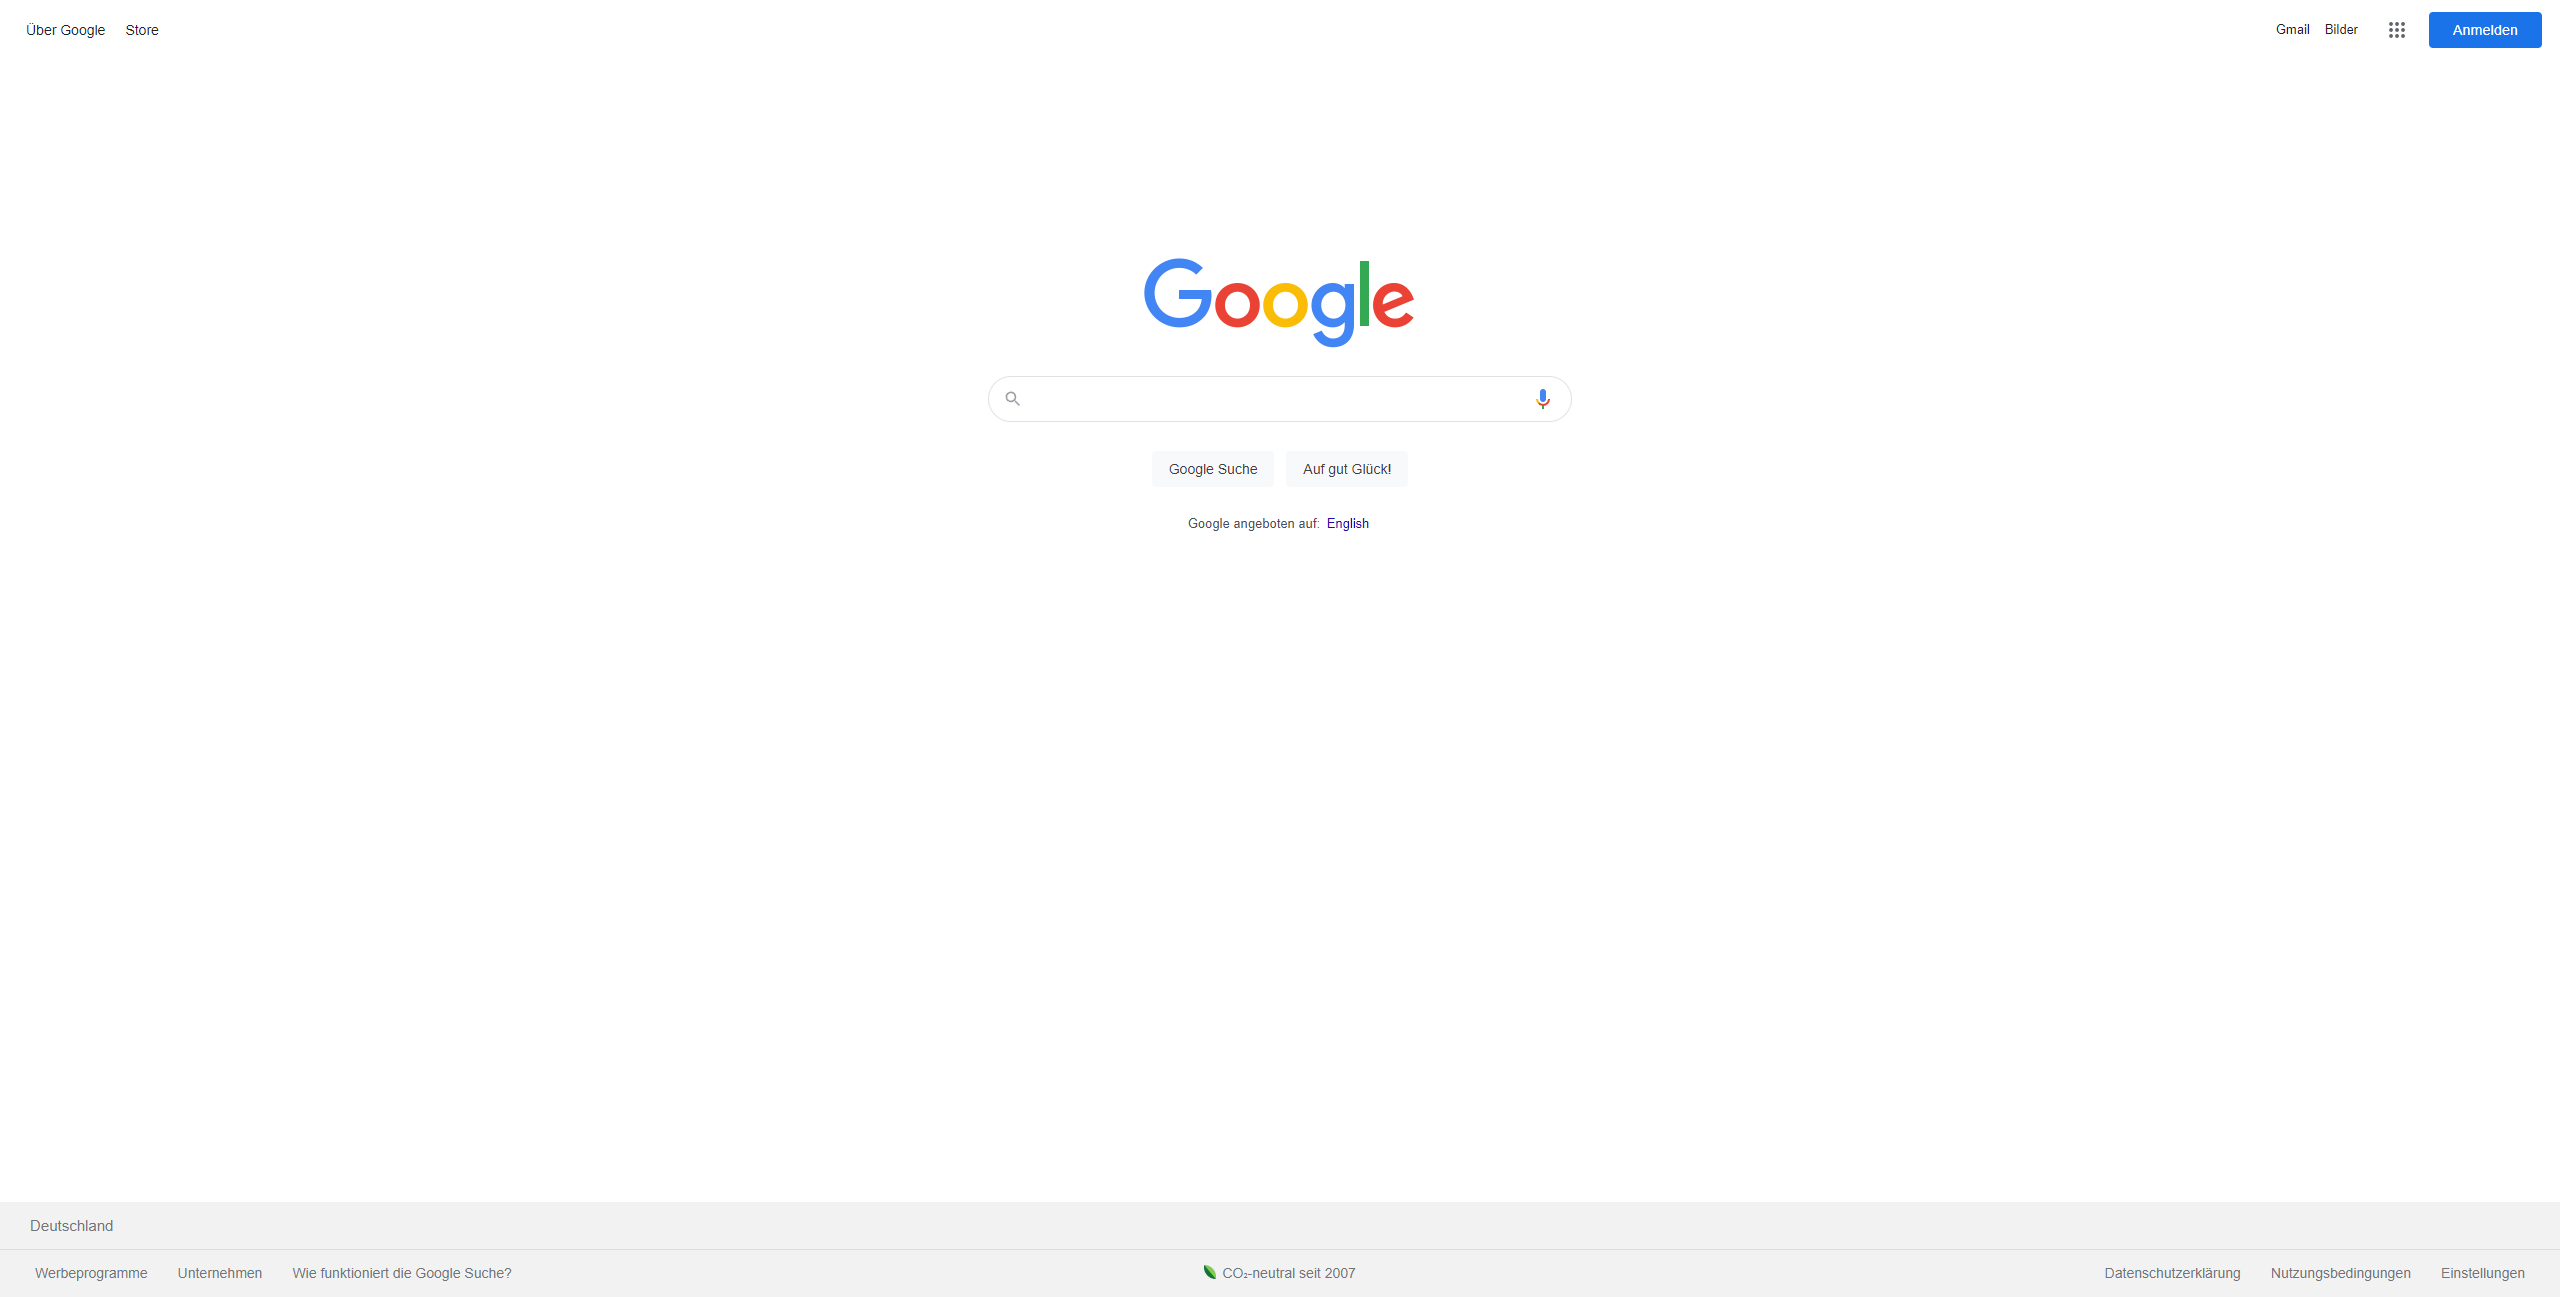
\includegraphics[height=0.3\textheight]{google_home}}\caption{Google Home}\label{fig:google_home}
    \fbox{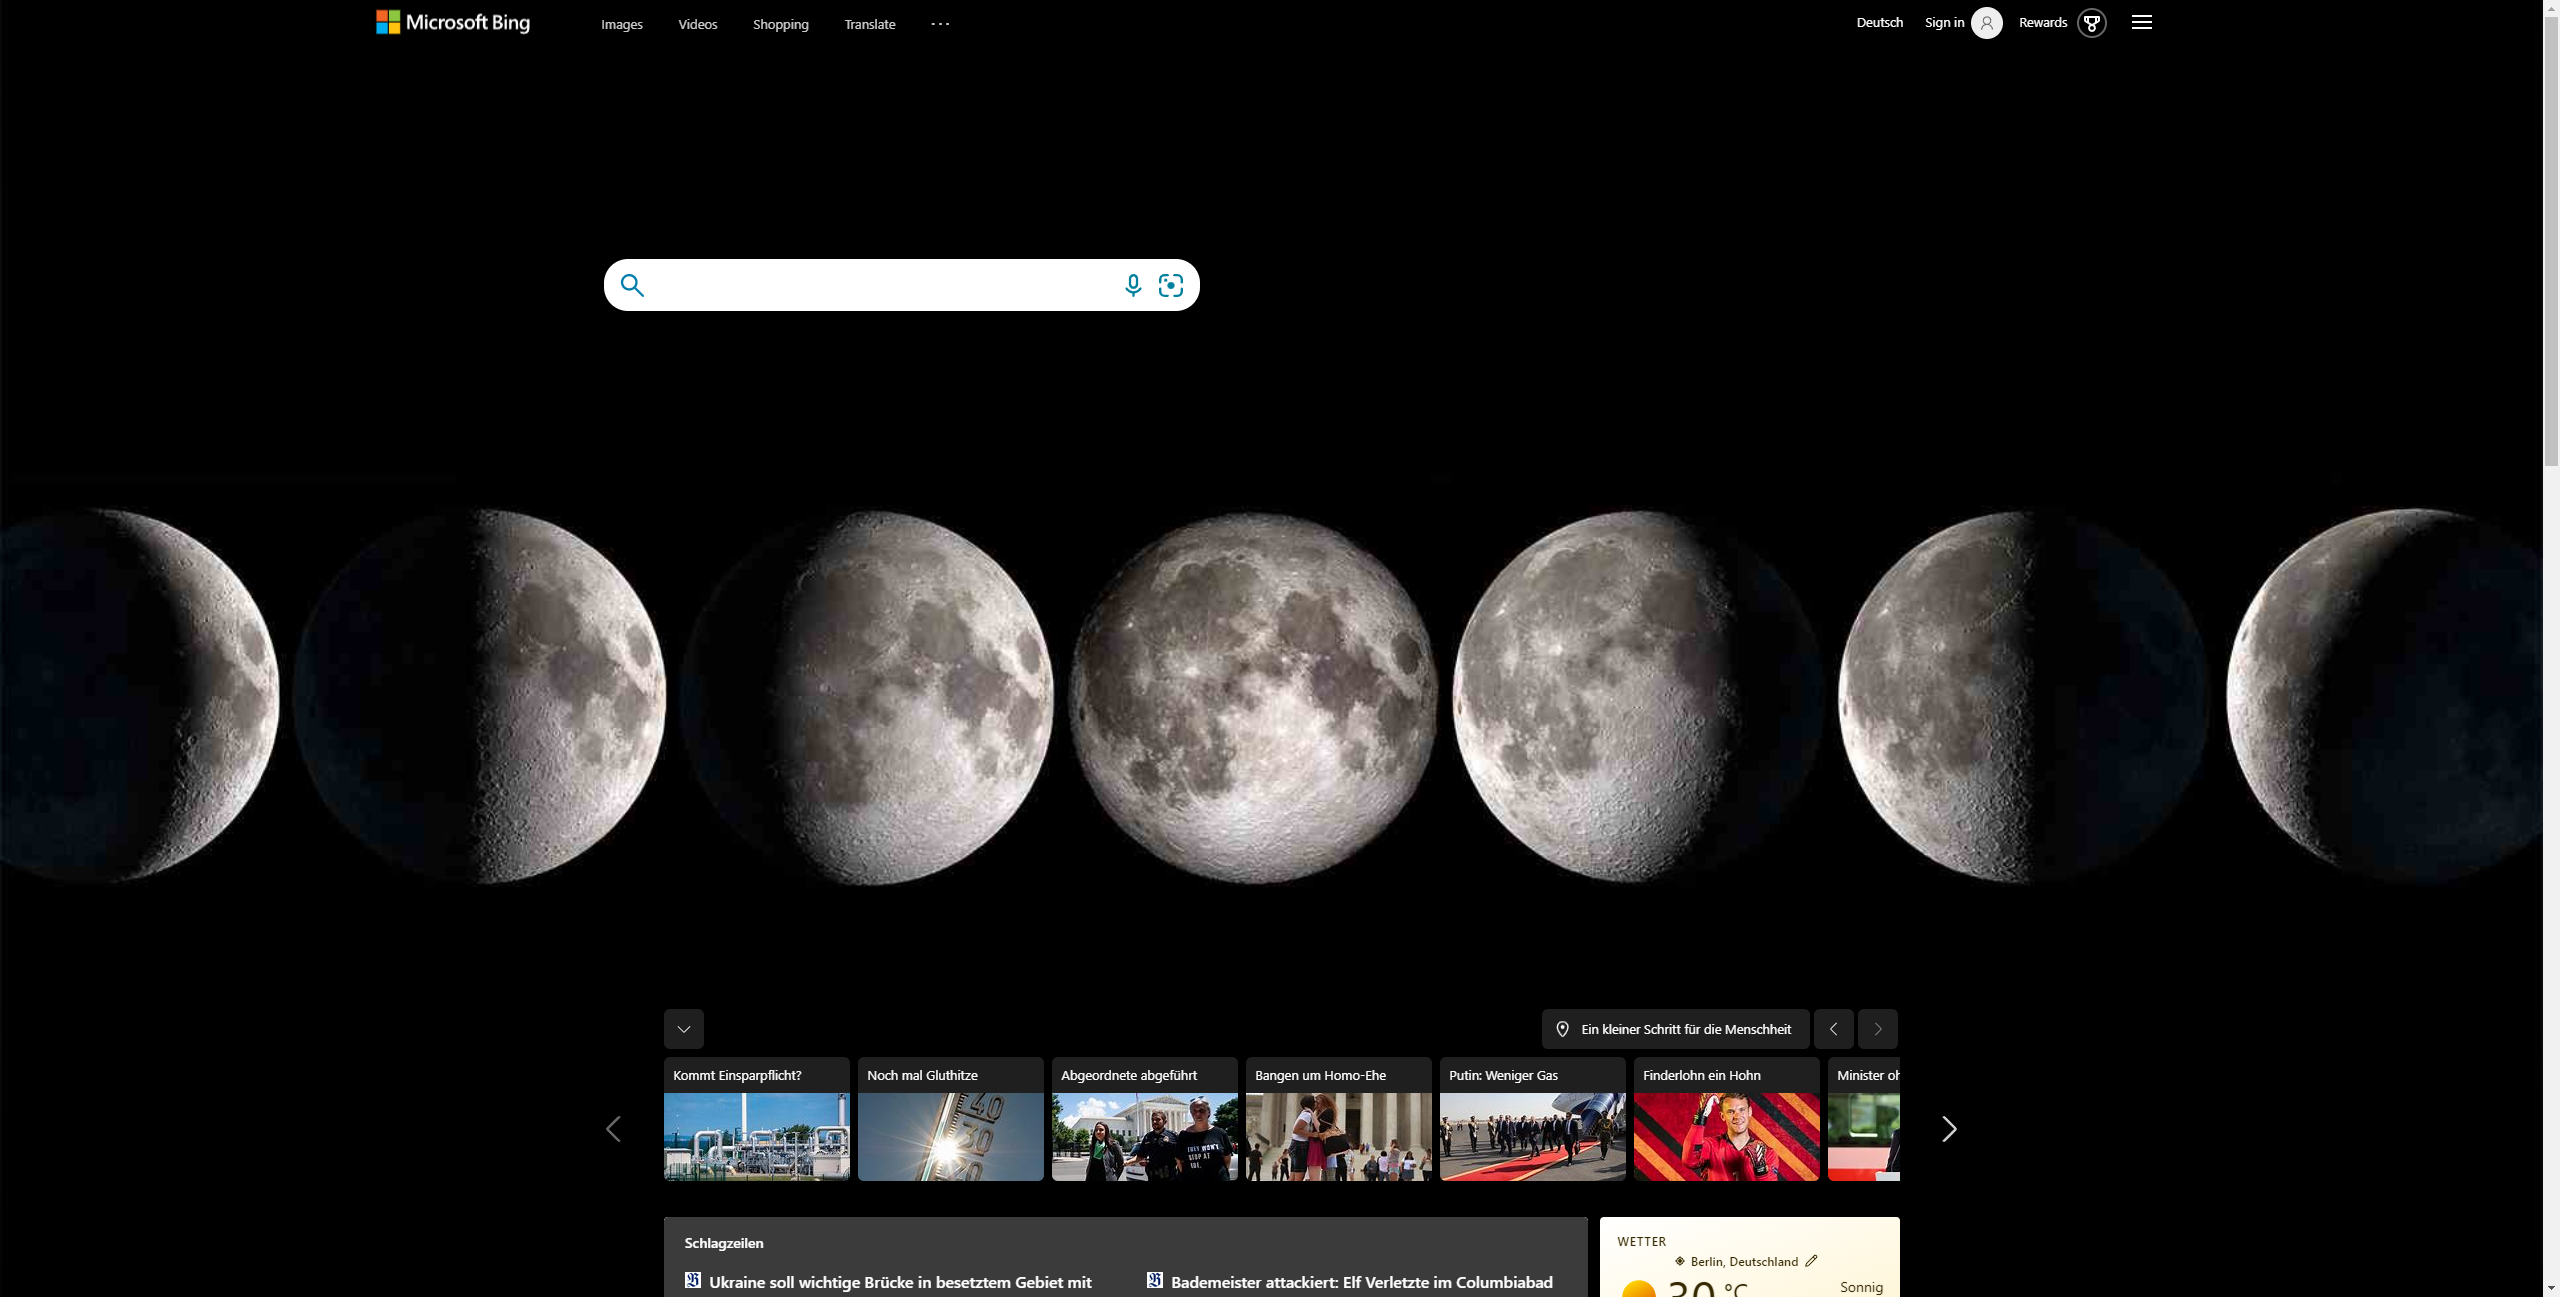
\includegraphics[height=0.3\textheight]{bing_home}}\caption{Bing Home}\label{fig:bing_home}
    \fbox{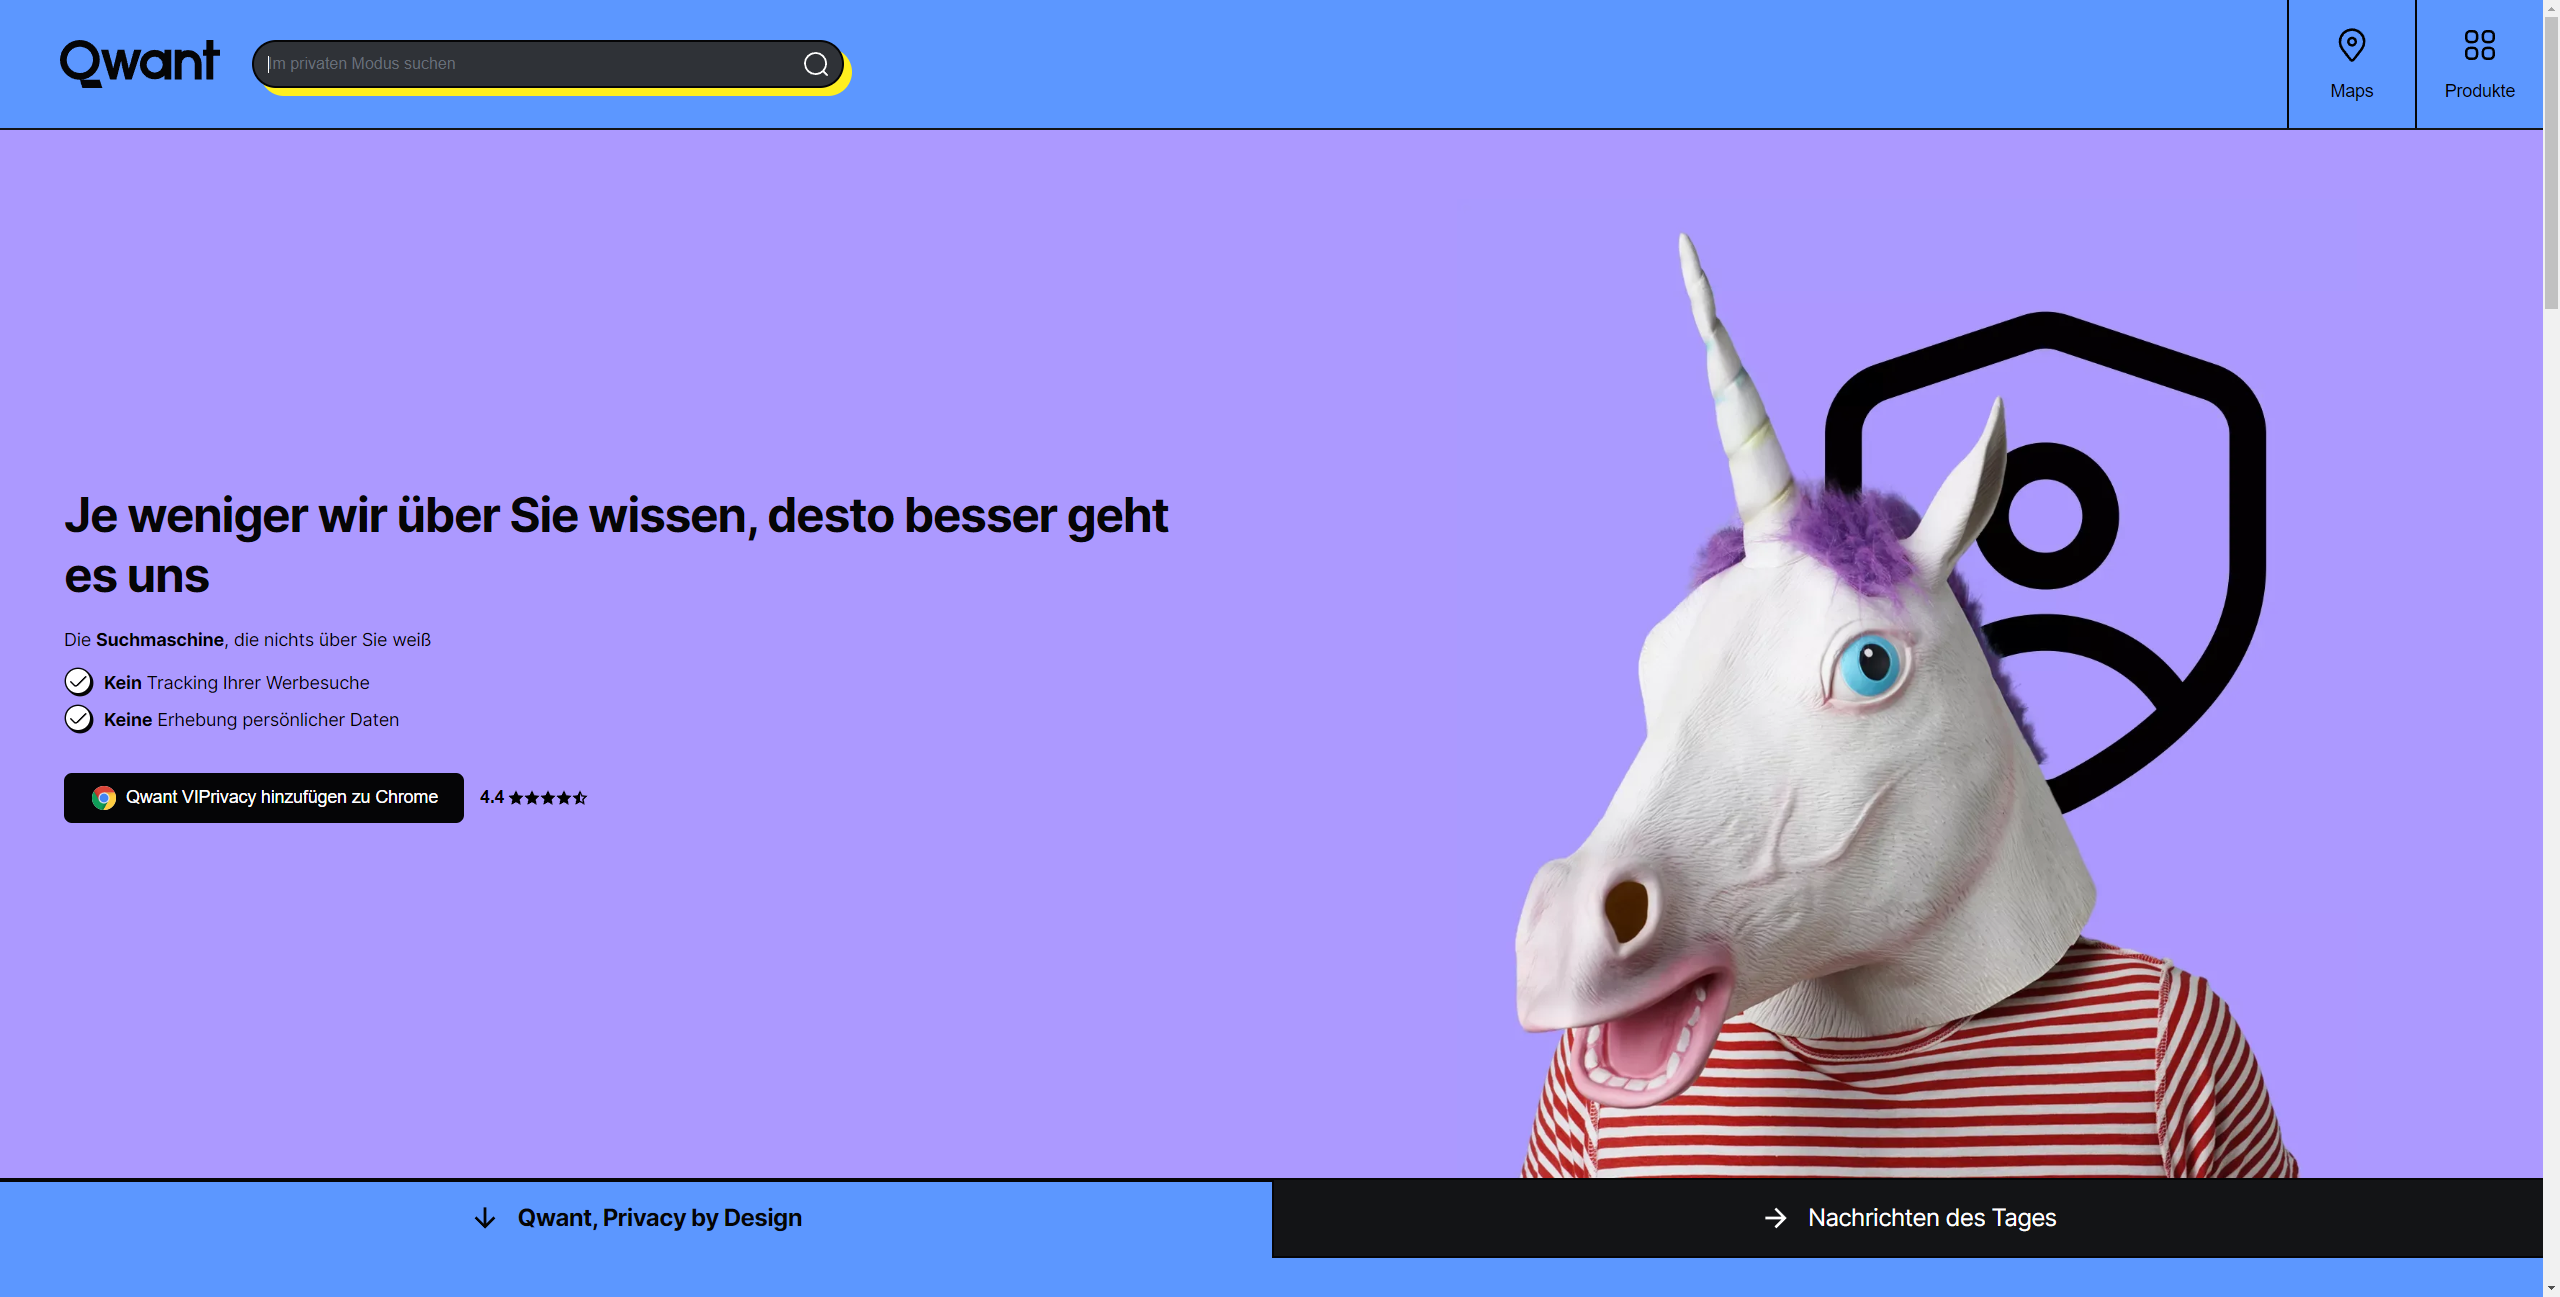
\includegraphics[height=0.3\textheight]{qwant_home}}\caption{Qwant Home}\label{fig:qwant_home}
\end{figure}
